
% Default to the notebook output style

    


% Inherit from the specified cell style.




    
\documentclass[11pt]{article}

    
    
    \usepackage[T1]{fontenc}
    % Nicer default font (+ math font) than Computer Modern for most use cases
    \usepackage{mathpazo}

    % Basic figure setup, for now with no caption control since it's done
    % automatically by Pandoc (which extracts ![](path) syntax from Markdown).
    \usepackage{graphicx}
    % We will generate all images so they have a width \maxwidth. This means
    % that they will get their normal width if they fit onto the page, but
    % are scaled down if they would overflow the margins.
    \makeatletter
    \def\maxwidth{\ifdim\Gin@nat@width>\linewidth\linewidth
    \else\Gin@nat@width\fi}
    \makeatother
    \let\Oldincludegraphics\includegraphics
    % Set max figure width to be 80% of text width, for now hardcoded.
    \renewcommand{\includegraphics}[1]{\Oldincludegraphics[width=.8\maxwidth]{#1}}
    % Ensure that by default, figures have no caption (until we provide a
    % proper Figure object with a Caption API and a way to capture that
    % in the conversion process - todo).
    \usepackage{caption}
    \DeclareCaptionLabelFormat{nolabel}{}
    \captionsetup{labelformat=nolabel}

    \usepackage{adjustbox} % Used to constrain images to a maximum size 
    \usepackage{xcolor} % Allow colors to be defined
    \usepackage{enumerate} % Needed for markdown enumerations to work
    \usepackage{geometry} % Used to adjust the document margins
    \usepackage{amsmath} % Equations
    \usepackage{amssymb} % Equations
    \usepackage{textcomp} % defines textquotesingle
    % Hack from http://tex.stackexchange.com/a/47451/13684:
    \AtBeginDocument{%
        \def\PYZsq{\textquotesingle}% Upright quotes in Pygmentized code
    }
    \usepackage{upquote} % Upright quotes for verbatim code
    \usepackage{eurosym} % defines \euro
    \usepackage[mathletters]{ucs} % Extended unicode (utf-8) support
    \usepackage[utf8x]{inputenc} % Allow utf-8 characters in the tex document
    \usepackage{fancyvrb} % verbatim replacement that allows latex
    \usepackage{grffile} % extends the file name processing of package graphics 
                         % to support a larger range 
    % The hyperref package gives us a pdf with properly built
    % internal navigation ('pdf bookmarks' for the table of contents,
    % internal cross-reference links, web links for URLs, etc.)
    \usepackage{hyperref}
    \usepackage{longtable} % longtable support required by pandoc >1.10
    \usepackage{booktabs}  % table support for pandoc > 1.12.2
    \usepackage[inline]{enumitem} % IRkernel/repr support (it uses the enumerate* environment)
    \usepackage[normalem]{ulem} % ulem is needed to support strikethroughs (\sout)
                                % normalem makes italics be italics, not underlines
    

    
    
    % Colors for the hyperref package
    \definecolor{urlcolor}{rgb}{0,.145,.698}
    \definecolor{linkcolor}{rgb}{.71,0.21,0.01}
    \definecolor{citecolor}{rgb}{.12,.54,.11}

    % ANSI colors
    \definecolor{ansi-black}{HTML}{3E424D}
    \definecolor{ansi-black-intense}{HTML}{282C36}
    \definecolor{ansi-red}{HTML}{E75C58}
    \definecolor{ansi-red-intense}{HTML}{B22B31}
    \definecolor{ansi-green}{HTML}{00A250}
    \definecolor{ansi-green-intense}{HTML}{007427}
    \definecolor{ansi-yellow}{HTML}{DDB62B}
    \definecolor{ansi-yellow-intense}{HTML}{B27D12}
    \definecolor{ansi-blue}{HTML}{208FFB}
    \definecolor{ansi-blue-intense}{HTML}{0065CA}
    \definecolor{ansi-magenta}{HTML}{D160C4}
    \definecolor{ansi-magenta-intense}{HTML}{A03196}
    \definecolor{ansi-cyan}{HTML}{60C6C8}
    \definecolor{ansi-cyan-intense}{HTML}{258F8F}
    \definecolor{ansi-white}{HTML}{C5C1B4}
    \definecolor{ansi-white-intense}{HTML}{A1A6B2}

    % commands and environments needed by pandoc snippets
    % extracted from the output of `pandoc -s`
    \providecommand{\tightlist}{%
      \setlength{\itemsep}{0pt}\setlength{\parskip}{0pt}}
    \DefineVerbatimEnvironment{Highlighting}{Verbatim}{commandchars=\\\{\}}
    % Add ',fontsize=\small' for more characters per line
    \newenvironment{Shaded}{}{}
    \newcommand{\KeywordTok}[1]{\textcolor[rgb]{0.00,0.44,0.13}{\textbf{{#1}}}}
    \newcommand{\DataTypeTok}[1]{\textcolor[rgb]{0.56,0.13,0.00}{{#1}}}
    \newcommand{\DecValTok}[1]{\textcolor[rgb]{0.25,0.63,0.44}{{#1}}}
    \newcommand{\BaseNTok}[1]{\textcolor[rgb]{0.25,0.63,0.44}{{#1}}}
    \newcommand{\FloatTok}[1]{\textcolor[rgb]{0.25,0.63,0.44}{{#1}}}
    \newcommand{\CharTok}[1]{\textcolor[rgb]{0.25,0.44,0.63}{{#1}}}
    \newcommand{\StringTok}[1]{\textcolor[rgb]{0.25,0.44,0.63}{{#1}}}
    \newcommand{\CommentTok}[1]{\textcolor[rgb]{0.38,0.63,0.69}{\textit{{#1}}}}
    \newcommand{\OtherTok}[1]{\textcolor[rgb]{0.00,0.44,0.13}{{#1}}}
    \newcommand{\AlertTok}[1]{\textcolor[rgb]{1.00,0.00,0.00}{\textbf{{#1}}}}
    \newcommand{\FunctionTok}[1]{\textcolor[rgb]{0.02,0.16,0.49}{{#1}}}
    \newcommand{\RegionMarkerTok}[1]{{#1}}
    \newcommand{\ErrorTok}[1]{\textcolor[rgb]{1.00,0.00,0.00}{\textbf{{#1}}}}
    \newcommand{\NormalTok}[1]{{#1}}
    
    % Additional commands for more recent versions of Pandoc
    \newcommand{\ConstantTok}[1]{\textcolor[rgb]{0.53,0.00,0.00}{{#1}}}
    \newcommand{\SpecialCharTok}[1]{\textcolor[rgb]{0.25,0.44,0.63}{{#1}}}
    \newcommand{\VerbatimStringTok}[1]{\textcolor[rgb]{0.25,0.44,0.63}{{#1}}}
    \newcommand{\SpecialStringTok}[1]{\textcolor[rgb]{0.73,0.40,0.53}{{#1}}}
    \newcommand{\ImportTok}[1]{{#1}}
    \newcommand{\DocumentationTok}[1]{\textcolor[rgb]{0.73,0.13,0.13}{\textit{{#1}}}}
    \newcommand{\AnnotationTok}[1]{\textcolor[rgb]{0.38,0.63,0.69}{\textbf{\textit{{#1}}}}}
    \newcommand{\CommentVarTok}[1]{\textcolor[rgb]{0.38,0.63,0.69}{\textbf{\textit{{#1}}}}}
    \newcommand{\VariableTok}[1]{\textcolor[rgb]{0.10,0.09,0.49}{{#1}}}
    \newcommand{\ControlFlowTok}[1]{\textcolor[rgb]{0.00,0.44,0.13}{\textbf{{#1}}}}
    \newcommand{\OperatorTok}[1]{\textcolor[rgb]{0.40,0.40,0.40}{{#1}}}
    \newcommand{\BuiltInTok}[1]{{#1}}
    \newcommand{\ExtensionTok}[1]{{#1}}
    \newcommand{\PreprocessorTok}[1]{\textcolor[rgb]{0.74,0.48,0.00}{{#1}}}
    \newcommand{\AttributeTok}[1]{\textcolor[rgb]{0.49,0.56,0.16}{{#1}}}
    \newcommand{\InformationTok}[1]{\textcolor[rgb]{0.38,0.63,0.69}{\textbf{\textit{{#1}}}}}
    \newcommand{\WarningTok}[1]{\textcolor[rgb]{0.38,0.63,0.69}{\textbf{\textit{{#1}}}}}
    
    
    % Define a nice break command that doesn't care if a line doesn't already
    % exist.
    \def\br{\hspace*{\fill} \\* }
    % Math Jax compatability definitions
    \def\gt{>}
    \def\lt{<}
    % Document parameters
    \title{lecture\_13}
    
    
    

    % Pygments definitions
    
\makeatletter
\def\PY@reset{\let\PY@it=\relax \let\PY@bf=\relax%
    \let\PY@ul=\relax \let\PY@tc=\relax%
    \let\PY@bc=\relax \let\PY@ff=\relax}
\def\PY@tok#1{\csname PY@tok@#1\endcsname}
\def\PY@toks#1+{\ifx\relax#1\empty\else%
    \PY@tok{#1}\expandafter\PY@toks\fi}
\def\PY@do#1{\PY@bc{\PY@tc{\PY@ul{%
    \PY@it{\PY@bf{\PY@ff{#1}}}}}}}
\def\PY#1#2{\PY@reset\PY@toks#1+\relax+\PY@do{#2}}

\expandafter\def\csname PY@tok@gd\endcsname{\def\PY@tc##1{\textcolor[rgb]{0.63,0.00,0.00}{##1}}}
\expandafter\def\csname PY@tok@gu\endcsname{\let\PY@bf=\textbf\def\PY@tc##1{\textcolor[rgb]{0.50,0.00,0.50}{##1}}}
\expandafter\def\csname PY@tok@gt\endcsname{\def\PY@tc##1{\textcolor[rgb]{0.00,0.27,0.87}{##1}}}
\expandafter\def\csname PY@tok@gs\endcsname{\let\PY@bf=\textbf}
\expandafter\def\csname PY@tok@gr\endcsname{\def\PY@tc##1{\textcolor[rgb]{1.00,0.00,0.00}{##1}}}
\expandafter\def\csname PY@tok@cm\endcsname{\let\PY@it=\textit\def\PY@tc##1{\textcolor[rgb]{0.25,0.50,0.50}{##1}}}
\expandafter\def\csname PY@tok@vg\endcsname{\def\PY@tc##1{\textcolor[rgb]{0.10,0.09,0.49}{##1}}}
\expandafter\def\csname PY@tok@vi\endcsname{\def\PY@tc##1{\textcolor[rgb]{0.10,0.09,0.49}{##1}}}
\expandafter\def\csname PY@tok@mh\endcsname{\def\PY@tc##1{\textcolor[rgb]{0.40,0.40,0.40}{##1}}}
\expandafter\def\csname PY@tok@cs\endcsname{\let\PY@it=\textit\def\PY@tc##1{\textcolor[rgb]{0.25,0.50,0.50}{##1}}}
\expandafter\def\csname PY@tok@ge\endcsname{\let\PY@it=\textit}
\expandafter\def\csname PY@tok@vc\endcsname{\def\PY@tc##1{\textcolor[rgb]{0.10,0.09,0.49}{##1}}}
\expandafter\def\csname PY@tok@il\endcsname{\def\PY@tc##1{\textcolor[rgb]{0.40,0.40,0.40}{##1}}}
\expandafter\def\csname PY@tok@go\endcsname{\def\PY@tc##1{\textcolor[rgb]{0.53,0.53,0.53}{##1}}}
\expandafter\def\csname PY@tok@cp\endcsname{\def\PY@tc##1{\textcolor[rgb]{0.74,0.48,0.00}{##1}}}
\expandafter\def\csname PY@tok@gi\endcsname{\def\PY@tc##1{\textcolor[rgb]{0.00,0.63,0.00}{##1}}}
\expandafter\def\csname PY@tok@gh\endcsname{\let\PY@bf=\textbf\def\PY@tc##1{\textcolor[rgb]{0.00,0.00,0.50}{##1}}}
\expandafter\def\csname PY@tok@ni\endcsname{\let\PY@bf=\textbf\def\PY@tc##1{\textcolor[rgb]{0.60,0.60,0.60}{##1}}}
\expandafter\def\csname PY@tok@nl\endcsname{\def\PY@tc##1{\textcolor[rgb]{0.63,0.63,0.00}{##1}}}
\expandafter\def\csname PY@tok@nn\endcsname{\let\PY@bf=\textbf\def\PY@tc##1{\textcolor[rgb]{0.00,0.00,1.00}{##1}}}
\expandafter\def\csname PY@tok@no\endcsname{\def\PY@tc##1{\textcolor[rgb]{0.53,0.00,0.00}{##1}}}
\expandafter\def\csname PY@tok@na\endcsname{\def\PY@tc##1{\textcolor[rgb]{0.49,0.56,0.16}{##1}}}
\expandafter\def\csname PY@tok@nb\endcsname{\def\PY@tc##1{\textcolor[rgb]{0.00,0.50,0.00}{##1}}}
\expandafter\def\csname PY@tok@nc\endcsname{\let\PY@bf=\textbf\def\PY@tc##1{\textcolor[rgb]{0.00,0.00,1.00}{##1}}}
\expandafter\def\csname PY@tok@nd\endcsname{\def\PY@tc##1{\textcolor[rgb]{0.67,0.13,1.00}{##1}}}
\expandafter\def\csname PY@tok@ne\endcsname{\let\PY@bf=\textbf\def\PY@tc##1{\textcolor[rgb]{0.82,0.25,0.23}{##1}}}
\expandafter\def\csname PY@tok@nf\endcsname{\def\PY@tc##1{\textcolor[rgb]{0.00,0.00,1.00}{##1}}}
\expandafter\def\csname PY@tok@si\endcsname{\let\PY@bf=\textbf\def\PY@tc##1{\textcolor[rgb]{0.73,0.40,0.53}{##1}}}
\expandafter\def\csname PY@tok@s2\endcsname{\def\PY@tc##1{\textcolor[rgb]{0.73,0.13,0.13}{##1}}}
\expandafter\def\csname PY@tok@nt\endcsname{\let\PY@bf=\textbf\def\PY@tc##1{\textcolor[rgb]{0.00,0.50,0.00}{##1}}}
\expandafter\def\csname PY@tok@nv\endcsname{\def\PY@tc##1{\textcolor[rgb]{0.10,0.09,0.49}{##1}}}
\expandafter\def\csname PY@tok@s1\endcsname{\def\PY@tc##1{\textcolor[rgb]{0.73,0.13,0.13}{##1}}}
\expandafter\def\csname PY@tok@ch\endcsname{\let\PY@it=\textit\def\PY@tc##1{\textcolor[rgb]{0.25,0.50,0.50}{##1}}}
\expandafter\def\csname PY@tok@m\endcsname{\def\PY@tc##1{\textcolor[rgb]{0.40,0.40,0.40}{##1}}}
\expandafter\def\csname PY@tok@gp\endcsname{\let\PY@bf=\textbf\def\PY@tc##1{\textcolor[rgb]{0.00,0.00,0.50}{##1}}}
\expandafter\def\csname PY@tok@sh\endcsname{\def\PY@tc##1{\textcolor[rgb]{0.73,0.13,0.13}{##1}}}
\expandafter\def\csname PY@tok@ow\endcsname{\let\PY@bf=\textbf\def\PY@tc##1{\textcolor[rgb]{0.67,0.13,1.00}{##1}}}
\expandafter\def\csname PY@tok@sx\endcsname{\def\PY@tc##1{\textcolor[rgb]{0.00,0.50,0.00}{##1}}}
\expandafter\def\csname PY@tok@bp\endcsname{\def\PY@tc##1{\textcolor[rgb]{0.00,0.50,0.00}{##1}}}
\expandafter\def\csname PY@tok@c1\endcsname{\let\PY@it=\textit\def\PY@tc##1{\textcolor[rgb]{0.25,0.50,0.50}{##1}}}
\expandafter\def\csname PY@tok@o\endcsname{\def\PY@tc##1{\textcolor[rgb]{0.40,0.40,0.40}{##1}}}
\expandafter\def\csname PY@tok@kc\endcsname{\let\PY@bf=\textbf\def\PY@tc##1{\textcolor[rgb]{0.00,0.50,0.00}{##1}}}
\expandafter\def\csname PY@tok@c\endcsname{\let\PY@it=\textit\def\PY@tc##1{\textcolor[rgb]{0.25,0.50,0.50}{##1}}}
\expandafter\def\csname PY@tok@mf\endcsname{\def\PY@tc##1{\textcolor[rgb]{0.40,0.40,0.40}{##1}}}
\expandafter\def\csname PY@tok@err\endcsname{\def\PY@bc##1{\setlength{\fboxsep}{0pt}\fcolorbox[rgb]{1.00,0.00,0.00}{1,1,1}{\strut ##1}}}
\expandafter\def\csname PY@tok@mb\endcsname{\def\PY@tc##1{\textcolor[rgb]{0.40,0.40,0.40}{##1}}}
\expandafter\def\csname PY@tok@ss\endcsname{\def\PY@tc##1{\textcolor[rgb]{0.10,0.09,0.49}{##1}}}
\expandafter\def\csname PY@tok@sr\endcsname{\def\PY@tc##1{\textcolor[rgb]{0.73,0.40,0.53}{##1}}}
\expandafter\def\csname PY@tok@mo\endcsname{\def\PY@tc##1{\textcolor[rgb]{0.40,0.40,0.40}{##1}}}
\expandafter\def\csname PY@tok@kd\endcsname{\let\PY@bf=\textbf\def\PY@tc##1{\textcolor[rgb]{0.00,0.50,0.00}{##1}}}
\expandafter\def\csname PY@tok@mi\endcsname{\def\PY@tc##1{\textcolor[rgb]{0.40,0.40,0.40}{##1}}}
\expandafter\def\csname PY@tok@kn\endcsname{\let\PY@bf=\textbf\def\PY@tc##1{\textcolor[rgb]{0.00,0.50,0.00}{##1}}}
\expandafter\def\csname PY@tok@cpf\endcsname{\let\PY@it=\textit\def\PY@tc##1{\textcolor[rgb]{0.25,0.50,0.50}{##1}}}
\expandafter\def\csname PY@tok@kr\endcsname{\let\PY@bf=\textbf\def\PY@tc##1{\textcolor[rgb]{0.00,0.50,0.00}{##1}}}
\expandafter\def\csname PY@tok@s\endcsname{\def\PY@tc##1{\textcolor[rgb]{0.73,0.13,0.13}{##1}}}
\expandafter\def\csname PY@tok@kp\endcsname{\def\PY@tc##1{\textcolor[rgb]{0.00,0.50,0.00}{##1}}}
\expandafter\def\csname PY@tok@w\endcsname{\def\PY@tc##1{\textcolor[rgb]{0.73,0.73,0.73}{##1}}}
\expandafter\def\csname PY@tok@kt\endcsname{\def\PY@tc##1{\textcolor[rgb]{0.69,0.00,0.25}{##1}}}
\expandafter\def\csname PY@tok@sc\endcsname{\def\PY@tc##1{\textcolor[rgb]{0.73,0.13,0.13}{##1}}}
\expandafter\def\csname PY@tok@sb\endcsname{\def\PY@tc##1{\textcolor[rgb]{0.73,0.13,0.13}{##1}}}
\expandafter\def\csname PY@tok@k\endcsname{\let\PY@bf=\textbf\def\PY@tc##1{\textcolor[rgb]{0.00,0.50,0.00}{##1}}}
\expandafter\def\csname PY@tok@se\endcsname{\let\PY@bf=\textbf\def\PY@tc##1{\textcolor[rgb]{0.73,0.40,0.13}{##1}}}
\expandafter\def\csname PY@tok@sd\endcsname{\let\PY@it=\textit\def\PY@tc##1{\textcolor[rgb]{0.73,0.13,0.13}{##1}}}

\def\PYZbs{\char`\\}
\def\PYZus{\char`\_}
\def\PYZob{\char`\{}
\def\PYZcb{\char`\}}
\def\PYZca{\char`\^}
\def\PYZam{\char`\&}
\def\PYZlt{\char`\<}
\def\PYZgt{\char`\>}
\def\PYZsh{\char`\#}
\def\PYZpc{\char`\%}
\def\PYZdl{\char`\$}
\def\PYZhy{\char`\-}
\def\PYZsq{\char`\'}
\def\PYZdq{\char`\"}
\def\PYZti{\char`\~}
% for compatibility with earlier versions
\def\PYZat{@}
\def\PYZlb{[}
\def\PYZrb{]}
\makeatother


    % Exact colors from NB
    \definecolor{incolor}{rgb}{0.0, 0.0, 0.5}
    \definecolor{outcolor}{rgb}{0.545, 0.0, 0.0}



    
    % Prevent overflowing lines due to hard-to-break entities
    \sloppy 
    % Setup hyperref package
    \hypersetup{
      breaklinks=true,  % so long urls are correctly broken across lines
      colorlinks=true,
      urlcolor=urlcolor,
      linkcolor=linkcolor,
      citecolor=citecolor,
      }
    % Slightly bigger margins than the latex defaults
    
    \geometry{verbose,tmargin=1in,bmargin=1in,lmargin=1in,rmargin=1in}
    
    

    \begin{document}
    
    
    \maketitle
    
    

    
    \begin{Verbatim}[commandchars=\\\{\}]
{\color{incolor}In [{\color{incolor}1}]:} \PY{c}{\PYZpc{}plot \PYZhy{}\PYZhy{}format svg}
\end{Verbatim}

    \begin{Verbatim}[commandchars=\\\{\}]
{\color{incolor}In [{\color{incolor}2}]:} \PY{n}{setdefaults}
\end{Verbatim}

    \subsection{My question from last
class}\label{my-question-from-last-class}

\begin{figure}[htbp]
\centering
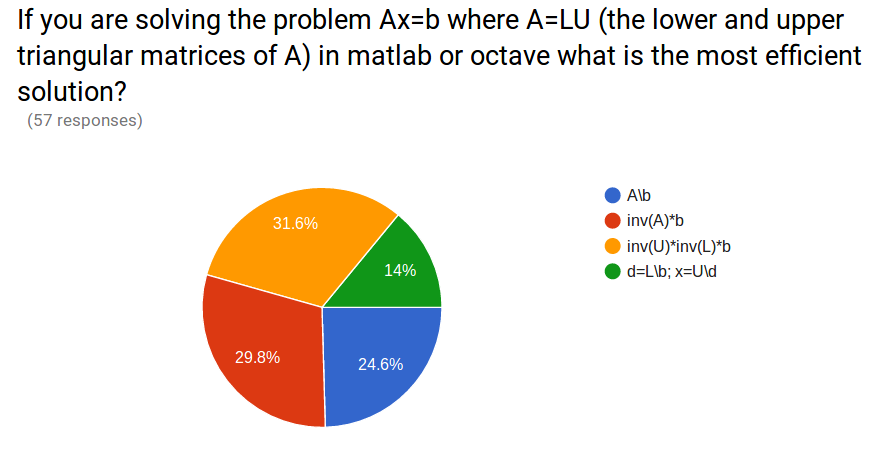
\includegraphics{efficient_soln.png}
\caption{q1}
\end{figure}

$A=\left[\begin{array}{ccc}
  2 & -2 & 0\\
  -1& 5 & 1 \\
3 &4 & 5 \end{array}\right]$

\begin{figure}[htbp]
\centering
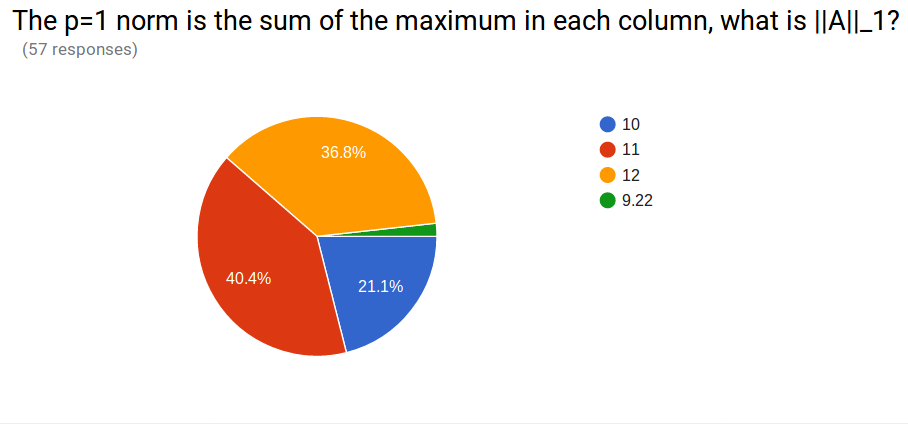
\includegraphics{norm_A.png}
\caption{q2}
\end{figure}

\subsection{Your questions from last
class}\label{your-questions-from-last-class}

\begin{enumerate}
\def\labelenumi{\arabic{enumi}.}
\item
  Do we have to submit a link for HW \#4 somewhere or is uploading to
  Github sufficient?

  -no, your submission from HW 3 is sufficient
\item
  How do I get the formulas/formatting in markdown files to show up on
  github?

  -no luck for markdown equations in github, this is an ongoing request
\item
  Confused about the p=1 norm part and
  \textbar{}\textbar{}A\textbar{}\textbar{}\_1
\item
  When's the exam?

  -next week (3/9)
\item
  What do you recommend doing to get better at figuring out the
  homeworks?

  -time and experimenting (try going through the lecture examples,
  verify my work)
\item
  Could we have an hw or extra credit with a video lecture to learn some
  simple python?

  -Sounds great! how simple?

  -\href{https://www.continuum.io/downloads}{Installing Python and
  Jupyter Notebook (via Anaconda) - https://www.continuum.io/downloads}

  -\href{https://anneurai.net/2015/11/12/matlab-based-ipython-notebooks/}{Running
  Matlab kernel in Jupyter -
  https://anneurai.net/2015/11/12/matlab-based-ipython-notebooks/}

  -\href{https://anaconda.org/pypi/octave_kernel}{Running Octave kernel
  in Jupyter - https://anaconda.org/pypi/octave\_kernel}
\end{enumerate}

    \subsection{Condition of a matrix}\label{condition-of-a-matrix}

\subsubsection{\texorpdfstring{\emph{just checked in to see what
condition my condition was
in}}{just checked in to see what condition my condition was in}}\label{just-checked-in-to-see-what-condition-my-condition-was-in}

\subsubsection{Matrix norms}\label{matrix-norms}

The Euclidean norm of a vector is measure of the magnitude (in 3D this
would be: $|x|=\sqrt{x_{1}^{2}+x_{2}^{2}+x_{3}^{2}}$) in general the
equation is:

$||x||_{e}=\sqrt{\sum_{i=1}^{n}x_{i}^{2}}$

For a matrix, A, the same norm is called the Frobenius norm:

$||A||_{f}=\sqrt{\sum_{i=1}^{n}\sum_{i=1}^{m}A_{i,j}^{2}}$

In general we can calculate any $p$-norm where

$||A||_{p}=\sqrt{\sum_{i=1}^{n}\sum_{i=1}^{m}A_{i,j}^{p}}$

so the p=1, 1-norm is

$||A||_{1}=\sqrt{\sum_{i=1}^{n}\sum_{i=1}^{m}A_{i,j}^{1}}=\sum_{i=1}^{n}\sum_{i=1}^{m}|A_{i,j}|$

$||A||_{\infty}=\sqrt{\sum_{i=1}^{n}\sum_{i=1}^{m}A_{i,j}^{\infty}}=\max_{1\le i \le n}\sum_{j=1}^{m}|A_{i,j}|$

\subsubsection{Condition of Matrix}\label{condition-of-matrix}

The matrix condition is the product of

$Cond(A) = ||A||\cdot||A^{-1}||$

So each norm will have a different condition number, but the limit is
$Cond(A)\ge 1$

An estimate of the rounding error is based on the condition of A:

$\frac{||\Delta x||}{x} \le Cond(A) \frac{||\Delta A||}{||A||}$

So if the coefficients of A have accuracy to \$10\^{}\{-t\}

and the condition of A, $Cond(A)=10^{c}$

then the solution for x can have rounding errors up to $10^{c-t}$

    \begin{Verbatim}[commandchars=\\\{\}]
{\color{incolor}In [{\color{incolor}72}]:} \PY{n}{A}\PY{p}{=}\PY{p}{[}\PY{l+m+mi}{1}\PY{p}{,}\PY{l+m+mi}{1}\PY{o}{/}\PY{l+m+mi}{2}\PY{p}{,}\PY{l+m+mi}{1}\PY{o}{/}\PY{l+m+mi}{3}\PY{p}{;}\PY{l+m+mi}{1}\PY{o}{/}\PY{l+m+mi}{2}\PY{p}{,}\PY{l+m+mi}{1}\PY{o}{/}\PY{l+m+mi}{3}\PY{p}{,}\PY{l+m+mi}{1}\PY{o}{/}\PY{l+m+mi}{4}\PY{p}{;}\PY{l+m+mi}{1}\PY{o}{/}\PY{l+m+mi}{3}\PY{p}{,}\PY{l+m+mi}{1}\PY{o}{/}\PY{l+m+mi}{4}\PY{p}{,}\PY{l+m+mi}{1}\PY{o}{/}\PY{l+m+mi}{5}\PY{p}{]}
         \PY{p}{[}\PY{n}{L}\PY{p}{,}\PY{n}{U}\PY{p}{]}\PY{p}{=}\PY{n}{LU\PYZus{}naive}\PY{p}{(}\PY{n}{A}\PY{p}{)}
\end{Verbatim}

    \begin{Verbatim}[commandchars=\\\{\}]
A =

   1.00000   0.50000   0.33333
   0.50000   0.33333   0.25000
   0.33333   0.25000   0.20000

L =

   1.00000   0.00000   0.00000
   0.50000   1.00000   0.00000
   0.33333   1.00000   1.00000

U =

   1.00000   0.50000   0.33333
   0.00000   0.08333   0.08333
   0.00000  -0.00000   0.00556


    \end{Verbatim}

    Then, $A^{-1}=(LU)^{-1}=U^{-1}L^{-1}$

$Ld_{1}=\left[\begin{array}{c} 1 \\ 0 \\ 0 \end{array}\right]$,
$Ux_{1}=d_{1}$ ...

    \begin{Verbatim}[commandchars=\\\{\}]
{\color{incolor}In [{\color{incolor}75}]:} \PY{n}{invA}\PY{p}{=}\PY{n+nb}{zeros}\PY{p}{(}\PY{l+m+mi}{3}\PY{p}{,}\PY{l+m+mi}{3}\PY{p}{)}\PY{p}{;}
         \PY{n}{d1}\PY{p}{=}\PY{n}{L}\PY{o}{\PYZbs{}}\PY{p}{[}\PY{l+m+mi}{1}\PY{p}{;}\PY{l+m+mi}{0}\PY{p}{;}\PY{l+m+mi}{0}\PY{p}{]}\PY{p}{;}
         \PY{n}{d2}\PY{p}{=}\PY{n}{L}\PY{o}{\PYZbs{}}\PY{p}{[}\PY{l+m+mi}{0}\PY{p}{;}\PY{l+m+mi}{1}\PY{p}{;}\PY{l+m+mi}{0}\PY{p}{]}\PY{p}{;}
         \PY{n}{d3}\PY{p}{=}\PY{n}{L}\PY{o}{\PYZbs{}}\PY{p}{[}\PY{l+m+mi}{0}\PY{p}{;}\PY{l+m+mi}{0}\PY{p}{;}\PY{l+m+mi}{1}\PY{p}{]}\PY{p}{;}
         \PY{n}{invA}\PY{p}{(}\PY{p}{:}\PY{p}{,}\PY{l+m+mi}{1}\PY{p}{)}\PY{p}{=}\PY{n}{U}\PY{o}{\PYZbs{}}\PY{n}{d1}\PY{p}{;}
         \PY{n}{invA}\PY{p}{(}\PY{p}{:}\PY{p}{,}\PY{l+m+mi}{2}\PY{p}{)}\PY{p}{=}\PY{n}{U}\PY{o}{\PYZbs{}}\PY{n}{d2}\PY{p}{;}
         \PY{n}{invA}\PY{p}{(}\PY{p}{:}\PY{p}{,}\PY{l+m+mi}{3}\PY{p}{)}\PY{p}{=}\PY{n}{U}\PY{o}{\PYZbs{}}\PY{n}{d3}
         \PY{n}{invA}\PY{o}{*}\PY{n}{A}
\end{Verbatim}

    \begin{Verbatim}[commandchars=\\\{\}]
invA =

     9.0000   -36.0000    30.0000
   -36.0000   192.0000  -180.0000
    30.0000  -180.0000   180.0000

ans =

   1.0000e+00   3.5527e-15   2.9976e-15
  -1.3249e-14   1.0000e+00  -9.1038e-15
   8.5117e-15   7.1054e-15   1.0000e+00


    \end{Verbatim}

    Find the condition of A, $cond(A)$

    \begin{Verbatim}[commandchars=\\\{\}]
{\color{incolor}In [{\color{incolor}74}]:} \PY{c}{\PYZpc{} Frobenius norm}
         \PY{n}{normf\PYZus{}A} \PY{p}{=} \PY{n+nb}{sqrt}\PY{p}{(}\PY{n+nb}{sum}\PY{p}{(}\PY{n+nb}{sum}\PY{p}{(}\PY{n}{A}\PY{o}{.\PYZca{}}\PY{l+m+mi}{2}\PY{p}{)}\PY{p}{)}\PY{p}{)}
         \PY{n}{normf\PYZus{}invA} \PY{p}{=} \PY{n+nb}{sqrt}\PY{p}{(}\PY{n+nb}{sum}\PY{p}{(}\PY{n+nb}{sum}\PY{p}{(}\PY{n}{invA}\PY{o}{.\PYZca{}}\PY{l+m+mi}{2}\PY{p}{)}\PY{p}{)}\PY{p}{)}
         
         \PY{n}{cond\PYZus{}f\PYZus{}A} \PY{p}{=} \PY{n}{normf\PYZus{}A}\PY{o}{*}\PY{n}{normf\PYZus{}invA}
         
         \PY{n+nb}{norm}\PY{p}{(}\PY{n}{A}\PY{p}{,}\PY{l+s}{\PYZsq{}}\PY{l+s}{fro\PYZsq{}}\PY{p}{)}
         
         \PY{c}{\PYZpc{} p=1, column sum norm}
         \PY{n}{norm1\PYZus{}A} \PY{p}{=} \PY{n+nb}{max}\PY{p}{(}\PY{n+nb}{sum}\PY{p}{(}\PY{n}{A}\PY{p}{,}\PY{l+m+mi}{2}\PY{p}{)}\PY{p}{)}
         \PY{n}{norm1\PYZus{}invA} \PY{p}{=} \PY{n+nb}{max}\PY{p}{(}\PY{n+nb}{sum}\PY{p}{(}\PY{n}{invA}\PY{p}{,}\PY{l+m+mi}{2}\PY{p}{)}\PY{p}{)}
         \PY{n+nb}{norm}\PY{p}{(}\PY{n}{A}\PY{p}{,}\PY{l+m+mi}{1}\PY{p}{)}
         
         \PY{n}{cond\PYZus{}1\PYZus{}A}\PY{p}{=}\PY{n}{norm1\PYZus{}A}\PY{o}{*}\PY{n}{norm1\PYZus{}invA}
         
         \PY{c}{\PYZpc{} p=inf, row sum norm}
         \PY{n}{norminf\PYZus{}A} \PY{p}{=} \PY{n+nb}{max}\PY{p}{(}\PY{n+nb}{sum}\PY{p}{(}\PY{n}{A}\PY{p}{,}\PY{l+m+mi}{1}\PY{p}{)}\PY{p}{)}
         \PY{n}{norminf\PYZus{}invA} \PY{p}{=} \PY{n+nb}{max}\PY{p}{(}\PY{n+nb}{sum}\PY{p}{(}\PY{n}{invA}\PY{p}{,}\PY{l+m+mi}{1}\PY{p}{)}\PY{p}{)}
         \PY{n+nb}{norm}\PY{p}{(}\PY{n}{A}\PY{p}{,}\PY{n+nb}{inf}\PY{p}{)}
         
         \PY{n}{cond\PYZus{}inf\PYZus{}A}\PY{p}{=}\PY{n}{norminf\PYZus{}A}\PY{o}{*}\PY{n}{norminf\PYZus{}invA}
\end{Verbatim}

    \begin{Verbatim}[commandchars=\\\{\}]
normf\_A =  1.4136
normf\_invA =  372.21
cond\_f\_A =  526.16
ans =  1.4136
norm1\_A =  1.8333
norm1\_invA =  30.000
ans =  1.8333
cond\_1\_A =  55.000
norminf\_A =  1.8333
norminf\_invA =  30.000
ans =  1.8333
cond\_inf\_A =  55.000

    \end{Verbatim}

    Consider the problem again from the intro to Linear Algebra, 4 masses
are connected in series to 4 springs with spring constants $K_{i}$.
What does a high condition number mean for this problem?

\begin{figure}[htbp]
\centering
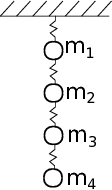
\includegraphics{../lecture_09/mass_springs.png}
\caption{Springs-masses}
\end{figure}

The masses haves the following amounts, 1, 2, 3, and 4 kg for masses
1-4. Using a FBD for each mass:

$m_{1}g+k_{2}(x_{2}-x_{1})-k_{1}x_{1}=0$

$m_{2}g+k_{3}(x_{3}-x_{2})-k_{2}(x_{2}-x_{1})=0$

$m_{3}g+k_{4}(x_{4}-x_{3})-k_{3}(x_{3}-x_{2})=0$

$m_{4}g-k_{4}(x_{4}-x_{3})=0$

in matrix form:

$\left[ \begin{array}{cccc} k_{1}+k_{2} & -k_{2} & 0 & 0 \\ -k_{2} & k_{2}+k_{3} & -k_{3} & 0 \\ 0 & -k_{3} & k_{3}+k_{4} & -k_{4} \\ 0 & 0 & -k_{4} & k_{4} \end{array} \right] \left[ \begin{array}{c} x_{1} \\ x_{2} \\ x_{3} \\ x_{4} \end{array} \right]= \left[ \begin{array}{c} m_{1}g \\ m_{2}g \\ m_{3}g \\ m_{4}g \end{array} \right]$

    \begin{Verbatim}[commandchars=\\\{\}]
{\color{incolor}In [{\color{incolor}21}]:} \PY{n}{k1}\PY{p}{=}\PY{l+m+mi}{10}\PY{p}{;} \PY{c}{\PYZpc{} N/m}
         \PY{n}{k2}\PY{p}{=}\PY{l+m+mi}{100000}\PY{p}{;}
         \PY{n}{k3}\PY{p}{=}\PY{l+m+mi}{10}\PY{p}{;}
         \PY{n}{k4}\PY{p}{=}\PY{l+m+mi}{1}\PY{p}{;}
         \PY{n}{m1}\PY{p}{=}\PY{l+m+mi}{1}\PY{p}{;} \PY{c}{\PYZpc{} kg}
         \PY{n}{m2}\PY{p}{=}\PY{l+m+mi}{2}\PY{p}{;}
         \PY{n}{m3}\PY{p}{=}\PY{l+m+mi}{3}\PY{p}{;}
         \PY{n}{m4}\PY{p}{=}\PY{l+m+mi}{4}\PY{p}{;}
         \PY{n}{g}\PY{p}{=}\PY{l+m+mf}{9.81}\PY{p}{;} \PY{c}{\PYZpc{} m/s\PYZca{}2}
         \PY{n}{K}\PY{p}{=}\PY{p}{[}\PY{n}{k1}\PY{o}{+}\PY{n}{k2} \PY{o}{\PYZhy{}}\PY{n}{k2} \PY{l+m+mi}{0} \PY{l+m+mi}{0}\PY{p}{;} \PY{o}{\PYZhy{}}\PY{n}{k2} \PY{n}{k2}\PY{o}{+}\PY{n}{k3} \PY{o}{\PYZhy{}}\PY{n}{k3} \PY{l+m+mi}{0}\PY{p}{;} \PY{l+m+mi}{0} \PY{o}{\PYZhy{}}\PY{n}{k3} \PY{n}{k3}\PY{o}{+}\PY{n}{k4} \PY{o}{\PYZhy{}}\PY{n}{k4}\PY{p}{;} \PY{l+m+mi}{0} \PY{l+m+mi}{0} \PY{o}{\PYZhy{}}\PY{n}{k4} \PY{n}{k4}\PY{p}{]}
         \PY{n}{y}\PY{p}{=}\PY{p}{[}\PY{n}{m1}\PY{o}{*}\PY{n}{g}\PY{p}{;}\PY{n}{m2}\PY{o}{*}\PY{n}{g}\PY{p}{;}\PY{n}{m3}\PY{o}{*}\PY{n}{g}\PY{p}{;}\PY{n}{m4}\PY{o}{*}\PY{n}{g}\PY{p}{]}
\end{Verbatim}

    \begin{Verbatim}[commandchars=\\\{\}]
K =

   100010  -100000        0        0
  -100000   100010      -10        0
        0      -10       11       -1
        0        0       -1        1

y =

    9.8100
   19.6200
   29.4300
   39.2400


    \end{Verbatim}

    \begin{Verbatim}[commandchars=\\\{\}]
{\color{incolor}In [{\color{incolor}25}]:} \PY{n+nb}{cond}\PY{p}{(}\PY{n}{K}\PY{p}{,}\PY{n+nb}{inf}\PY{p}{)}
         \PY{n+nb}{cond}\PY{p}{(}\PY{n}{K}\PY{p}{,}\PY{l+m+mi}{1}\PY{p}{)}
         \PY{n+nb}{cond}\PY{p}{(}\PY{n}{K}\PY{p}{,}\PY{l+s}{\PYZsq{}}\PY{l+s}{fro\PYZsq{}}\PY{p}{)}
         \PY{n+nb}{cond}\PY{p}{(}\PY{n}{K}\PY{p}{,}\PY{l+m+mi}{2}\PY{p}{)}
\end{Verbatim}

    \begin{Verbatim}[commandchars=\\\{\}]
ans =    3.2004e+05
ans =    3.2004e+05
ans =    2.5925e+05
ans =    2.5293e+05

    \end{Verbatim}

    \begin{Verbatim}[commandchars=\\\{\}]
{\color{incolor}In [{\color{incolor}26}]:} \PY{n+nb}{e}\PY{p}{=}\PY{n+nb}{eig}\PY{p}{(}\PY{n}{K}\PY{p}{)}
         \PY{n+nb}{max}\PY{p}{(}\PY{n+nb}{e}\PY{p}{)}\PY{o}{/}\PY{n+nb}{min}\PY{p}{(}\PY{n+nb}{e}\PY{p}{)}
\end{Verbatim}

    \begin{Verbatim}[commandchars=\\\{\}]
e =

   7.9078e-01
   3.5881e+00
   1.7621e+01
   2.0001e+05

ans =    2.5293e+05

    \end{Verbatim}

    \section{Iterative Methods}\label{iterative-methods}

\subsection{Gauss-Seidel method}\label{gauss-seidel-method}

If we have an intial guess for each value of a vector $x$ that we are
trying to solve, then it is easy enough to solve for one component given
the others.

Take a 3$\times$3 matrix

$Ax=b$

$\left[ \begin{array}{ccc} 3 & -0.1 & -0.2 \\ 0.1 & 7 & -0.3 \\ 0.3 & -0.2 & 10 \end{array} \right] \left[ \begin{array}{c} x_{1} \\ x_{2} \\ x_{3} \end{array} \right]= \left[ \begin{array}{c} 7.85 \\ -19.3 \\ 71.4\end{array} \right]$

$x_{1}=\frac{7.85+0.1x_{2}+0.3x_{3}}{3}$

$x_{2}=\frac{-19.3-0.1x_{1}+0.3x_{3}}{7}$

$x_{3}=\frac{71.4+0.1x_{1}+0.2x_{2}}{10}$

    \begin{Verbatim}[commandchars=\\\{\}]
{\color{incolor}In [{\color{incolor}9}]:} \PY{n}{A}\PY{p}{=}\PY{p}{[}\PY{l+m+mi}{3} \PY{o}{\PYZhy{}}\PY{l+m+mf}{0.1} \PY{o}{\PYZhy{}}\PY{l+m+mf}{0.2}\PY{p}{;}\PY{l+m+mf}{0.1} \PY{l+m+mi}{7} \PY{o}{\PYZhy{}}\PY{l+m+mf}{0.3}\PY{p}{;}\PY{l+m+mf}{0.3} \PY{o}{\PYZhy{}}\PY{l+m+mf}{0.2} \PY{l+m+mi}{10}\PY{p}{]}
        \PY{n}{b}\PY{p}{=}\PY{p}{[}\PY{l+m+mf}{7.85}\PY{p}{;}\PY{o}{\PYZhy{}}\PY{l+m+mf}{19.3}\PY{p}{;}\PY{l+m+mf}{71.4}\PY{p}{]}
        
        \PY{n}{x}\PY{p}{=}\PY{n}{A}\PY{o}{\PYZbs{}}\PY{n}{b}
\end{Verbatim}

    \begin{Verbatim}[commandchars=\\\{\}]
A =

    3.00000   -0.10000   -0.20000
    0.10000    7.00000   -0.30000
    0.30000   -0.20000   10.00000

b =

    7.8500
  -19.3000
   71.4000

x =

   3.0000
  -2.5000
   7.0000


    \end{Verbatim}

    \subsubsection{Gauss-Seidel Iterative
approach}\label{gauss-seidel-iterative-approach}

As a first guess, we can use $x_{1}=x_{2}=x_{3}=0$

$x_{1}=\frac{7.85+0.1(0)+0.3(0)}{3}=2.6167$

$x_{2}=\frac{-19.3-0.1(2.6167)+0.3(0)}{7}=-2.7945$

$x_{3}=\frac{71.4+0.1(2.6167)+0.2(-2.7945)}{10}=7.0056$

Then, we update the guess:

$x_{1}=\frac{7.85+0.1(-2.7945)+0.3(7.0056)}{3}=2.9906$

$x_{2}=\frac{-19.3-0.1(2.9906)+0.3(7.0056)}{7}=-2.4996$

$x_{3}=\frac{71.4+0.1(2.9906)+0.2(-2.4966)}{10}=7.00029$

The results are conveerging to the solution we found with
\texttt{\textbackslash{}} of $x_{1}=3,~x_{2}=-2.5,~x_{3}=7$

We could also use an iterative method that solves for all of the
x-components in one step:

\subsubsection{Jacobi method}\label{jacobi-method}

$x_{1}^{i}=\frac{7.85+0.1x_{2}^{i-1}+0.3x_{3}^{i-1}}{3}$

$x_{2}^{i}=\frac{-19.3-0.1x_{1}^{i-1}+0.3x_{3}^{i-1}}{7}$

$x_{3}^{i}=\frac{71.4+0.1x_{1}^{i-1}+0.2x_{2}^{i-1}}{10}$

Here the solution is a matrix multiplication and vector addition

$\left[ \begin{array}{c} x_{1}^{i} \\ x_{2}^{i} \\ x_{3}^{i} \end{array} \right]= \left[ \begin{array}{c} 7.85/3 \\ -19.3/7 \\ 71.4/10\end{array} \right]- \left[ \begin{array}{ccc} 0 & -0.1 & -0.2 \\ 0.1 & 0 & -0.3 \\ 0.3 & -0.2 & 0 \end{array} \right] \left[ \begin{array}{c} x_{1}^{i-1} \\ x_{2}^{i-1} \\ x_{3}^{i-1} \end{array} \right]$

\begin{longtable}[c]{@{}llll@{}}
\toprule
\begin{minipage}[b]{0.10\columnwidth}\raggedright\strut
x\_\{j\}
\strut\end{minipage} &
\begin{minipage}[b]{0.36\columnwidth}\raggedright\strut
Jacobi method
\strut\end{minipage} &
\begin{minipage}[b]{0.05\columnwidth}\raggedright\strut
vs
\strut\end{minipage} &
\begin{minipage}[b]{0.37\columnwidth}\raggedright\strut
Gauss-Seidel
\strut\end{minipage}\tabularnewline
\midrule
\endhead
\begin{minipage}[t]{0.10\columnwidth}\raggedright\strut
$x_{1}^{i}=$
\strut\end{minipage} &
\begin{minipage}[t]{0.36\columnwidth}\raggedright\strut
$\frac{7.85+0.1x_{2}^{i-1}+0.3x_{3}^{i-1}}{3}$
\strut\end{minipage} &
\begin{minipage}[t]{0.05\columnwidth}\raggedright\strut
\strut\end{minipage} &
\begin{minipage}[t]{0.37\columnwidth}\raggedright\strut
$\frac{7.85+0.1x_{2}^{i-1}+0.3x_{3}^{i-1}}{3}$
\strut\end{minipage}\tabularnewline
\begin{minipage}[t]{0.10\columnwidth}\raggedright\strut
$x_{2}^{i}=$
\strut\end{minipage} &
\begin{minipage}[t]{0.36\columnwidth}\raggedright\strut
$\frac{-19.3-0.1x_{1}^{i-1}+0.3x_{3}^{i-1}}{7}$
\strut\end{minipage} &
\begin{minipage}[t]{0.05\columnwidth}\raggedright\strut
\strut\end{minipage} &
\begin{minipage}[t]{0.37\columnwidth}\raggedright\strut
$\frac{-19.3-0.1x_{1}^{i}+0.3x_{3}^{i-1}}{7}$
\strut\end{minipage}\tabularnewline
\begin{minipage}[t]{0.10\columnwidth}\raggedright\strut
$x_{3}^{i}=$
\strut\end{minipage} &
\begin{minipage}[t]{0.36\columnwidth}\raggedright\strut
$\frac{71.4+0.1x_{1}^{i-1}+0.2x_{2}^{i-1}}{10}$
\strut\end{minipage} &
\begin{minipage}[t]{0.05\columnwidth}\raggedright\strut
\strut\end{minipage} &
\begin{minipage}[t]{0.37\columnwidth}\raggedright\strut
$\frac{71.4+0.1x_{1}^{i}+0.2x_{2}^{i}}{10}$
\strut\end{minipage}\tabularnewline
\bottomrule
\end{longtable}

    \begin{Verbatim}[commandchars=\\\{\}]
{\color{incolor}In [{\color{incolor}15}]:} \PY{n}{ba}\PY{p}{=}\PY{n}{b}\PY{o}{./}\PY{n+nb}{diag}\PY{p}{(}\PY{n}{A}\PY{p}{)} \PY{c}{\PYZpc{} or ba=b./[A(1,1);A(2,2);A(3,3)]}
         \PY{n}{sA}\PY{p}{=}\PY{n}{A}\PY{o}{\PYZhy{}}\PY{n+nb}{diag}\PY{p}{(}\PY{n+nb}{diag}\PY{p}{(}\PY{n}{A}\PY{p}{)}\PY{p}{)} \PY{c}{\PYZpc{} A with zeros on diagonal}
         \PY{n}{sA}\PY{p}{(}\PY{l+m+mi}{1}\PY{p}{,}\PY{p}{:}\PY{p}{)}\PY{p}{=}\PY{n}{sA}\PY{p}{(}\PY{l+m+mi}{1}\PY{p}{,}\PY{p}{:}\PY{p}{)}\PY{o}{/}\PY{n}{A}\PY{p}{(}\PY{l+m+mi}{1}\PY{p}{,}\PY{l+m+mi}{1}\PY{p}{)}\PY{p}{;}
         \PY{n}{sA}\PY{p}{(}\PY{l+m+mi}{2}\PY{p}{,}\PY{p}{:}\PY{p}{)}\PY{p}{=}\PY{n}{sA}\PY{p}{(}\PY{l+m+mi}{2}\PY{p}{,}\PY{p}{:}\PY{p}{)}\PY{o}{/}\PY{n}{A}\PY{p}{(}\PY{l+m+mi}{2}\PY{p}{,}\PY{l+m+mi}{2}\PY{p}{)}\PY{p}{;}
         \PY{n}{sA}\PY{p}{(}\PY{l+m+mi}{3}\PY{p}{,}\PY{p}{:}\PY{p}{)}\PY{p}{=}\PY{n}{sA}\PY{p}{(}\PY{l+m+mi}{3}\PY{p}{,}\PY{p}{:}\PY{p}{)}\PY{o}{/}\PY{n}{A}\PY{p}{(}\PY{l+m+mi}{3}\PY{p}{,}\PY{l+m+mi}{3}\PY{p}{)}
         \PY{n}{x0}\PY{p}{=}\PY{p}{[}\PY{l+m+mi}{0}\PY{p}{;}\PY{l+m+mi}{0}\PY{p}{;}\PY{l+m+mi}{0}\PY{p}{]}\PY{p}{;}
         \PY{n}{x1}\PY{p}{=}\PY{n}{ba}\PY{o}{\PYZhy{}}\PY{n}{sA}\PY{o}{*}\PY{n}{x0}
         \PY{n}{x2}\PY{p}{=}\PY{n}{ba}\PY{o}{\PYZhy{}}\PY{n}{sA}\PY{o}{*}\PY{n}{x1}
         \PY{n}{x3}\PY{p}{=}\PY{n}{ba}\PY{o}{\PYZhy{}}\PY{n}{sA}\PY{o}{*}\PY{n}{x2}
         \PY{n+nb}{fprintf}\PY{p}{(}\PY{l+s}{\PYZsq{}}\PY{l+s}{solution is converging to [3,\PYZhy{}2.5,7]]\PYZbs{}n\PYZsq{}}\PY{p}{)}
\end{Verbatim}

    \begin{Verbatim}[commandchars=\\\{\}]
ba =

   2.6167
  -2.7571
   7.1400

sA =

   0.00000  -0.10000  -0.20000
   0.10000   0.00000  -0.30000
   0.30000  -0.20000   0.00000

sA =

   0.000000  -0.033333  -0.066667
   0.014286   0.000000  -0.042857
   0.030000  -0.020000   0.000000

x1 =

   2.6167
  -2.7571
   7.1400

x2 =

   3.0008
  -2.4885
   7.0064

x3 =

   3.0008
  -2.4997
   7.0002

solution is converging to [3,-2.5,7]]

    \end{Verbatim}

    \begin{Verbatim}[commandchars=\\\{\}]
{\color{incolor}In [{\color{incolor}16}]:} \PY{n+nb}{diag}\PY{p}{(}\PY{n}{A}\PY{p}{)}
         \PY{n+nb}{diag}\PY{p}{(}\PY{n+nb}{diag}\PY{p}{(}\PY{n}{A}\PY{p}{)}\PY{p}{)}
\end{Verbatim}

    \begin{Verbatim}[commandchars=\\\{\}]
ans =

    3
    7
   10

ans =

Diagonal Matrix

    3    0    0
    0    7    0
    0    0   10


    \end{Verbatim}

    This method works if problem is diagonally dominant,

$|a_{ii}|>\sum_{j=1,j\ne i}^{n}|a_{ij}|$

If this condition is true, then Jacobi or Gauss-Seidel should converge

    \begin{Verbatim}[commandchars=\\\{\}]
{\color{incolor}In [{\color{incolor}17}]:} \PY{n}{A}\PY{p}{=}\PY{p}{[}\PY{l+m+mf}{0.1}\PY{p}{,}\PY{l+m+mi}{1}\PY{p}{,}\PY{l+m+mi}{3}\PY{p}{;}\PY{l+m+mi}{1}\PY{p}{,}\PY{l+m+mf}{0.2}\PY{p}{,}\PY{l+m+mi}{3}\PY{p}{;}\PY{l+m+mi}{5}\PY{p}{,}\PY{l+m+mi}{2}\PY{p}{,}\PY{l+m+mf}{0.3}\PY{p}{]}
         \PY{n}{b}\PY{p}{=}\PY{p}{[}\PY{l+m+mi}{12}\PY{p}{;}\PY{l+m+mi}{2}\PY{p}{;}\PY{l+m+mi}{4}\PY{p}{]}
         \PY{n}{A}\PY{o}{\PYZbs{}}\PY{n}{b}
\end{Verbatim}

    \begin{Verbatim}[commandchars=\\\{\}]
A =

   0.10000   1.00000   3.00000
   1.00000   0.20000   3.00000
   5.00000   2.00000   0.30000

b =

   12
    2
    4

ans =

  -2.9393
   9.1933
   1.0336


    \end{Verbatim}

    \begin{Verbatim}[commandchars=\\\{\}]
{\color{incolor}In [{\color{incolor}20}]:} \PY{n}{ba}\PY{p}{=}\PY{n}{b}\PY{o}{./}\PY{n+nb}{diag}\PY{p}{(}\PY{n}{A}\PY{p}{)} \PY{c}{\PYZpc{} or ba=b./[A(1,1);A(2,2);A(3,3)]}
         \PY{n}{sA}\PY{p}{=}\PY{n}{A}\PY{o}{\PYZhy{}}\PY{n+nb}{diag}\PY{p}{(}\PY{n+nb}{diag}\PY{p}{(}\PY{n}{A}\PY{p}{)}\PY{p}{)} \PY{c}{\PYZpc{} A with zeros on diagonal}
         \PY{n}{sA}\PY{p}{(}\PY{l+m+mi}{1}\PY{p}{,}\PY{p}{:}\PY{p}{)}\PY{p}{=}\PY{n}{sA}\PY{p}{(}\PY{l+m+mi}{1}\PY{p}{,}\PY{p}{:}\PY{p}{)}\PY{o}{/}\PY{n}{A}\PY{p}{(}\PY{l+m+mi}{1}\PY{p}{,}\PY{l+m+mi}{1}\PY{p}{)}\PY{p}{;}
         \PY{n}{sA}\PY{p}{(}\PY{l+m+mi}{2}\PY{p}{,}\PY{p}{:}\PY{p}{)}\PY{p}{=}\PY{n}{sA}\PY{p}{(}\PY{l+m+mi}{2}\PY{p}{,}\PY{p}{:}\PY{p}{)}\PY{o}{/}\PY{n}{A}\PY{p}{(}\PY{l+m+mi}{2}\PY{p}{,}\PY{l+m+mi}{2}\PY{p}{)}\PY{p}{;}
         \PY{n}{sA}\PY{p}{(}\PY{l+m+mi}{3}\PY{p}{,}\PY{p}{:}\PY{p}{)}\PY{p}{=}\PY{n}{sA}\PY{p}{(}\PY{l+m+mi}{3}\PY{p}{,}\PY{p}{:}\PY{p}{)}\PY{o}{/}\PY{n}{A}\PY{p}{(}\PY{l+m+mi}{3}\PY{p}{,}\PY{l+m+mi}{3}\PY{p}{)}
         \PY{n}{x0}\PY{p}{=}\PY{p}{[}\PY{l+m+mi}{0}\PY{p}{;}\PY{l+m+mi}{0}\PY{p}{;}\PY{l+m+mi}{0}\PY{p}{]}\PY{p}{;}
         \PY{n}{x1}\PY{p}{=}\PY{n}{ba}\PY{o}{\PYZhy{}}\PY{n}{sA}\PY{o}{*}\PY{n}{x0}
         \PY{n}{x2}\PY{p}{=}\PY{n}{ba}\PY{o}{\PYZhy{}}\PY{n}{sA}\PY{o}{*}\PY{n}{x1}
         \PY{n}{x3}\PY{p}{=}\PY{n}{ba}\PY{o}{\PYZhy{}}\PY{n}{sA}\PY{o}{*}\PY{n}{x2}
         \PY{n+nb}{fprintf}\PY{p}{(}\PY{l+s}{\PYZsq{}}\PY{l+s}{solution is not converging to [\PYZhy{}2.93,9.19,1.03]\PYZbs{}n\PYZsq{}}\PY{p}{)}
\end{Verbatim}

    \begin{Verbatim}[commandchars=\\\{\}]
ba =

   120.000
    10.000
    13.333

sA =

   0   1   3
   1   0   3
   5   2   0

sA =

    0.00000   10.00000   30.00000
    5.00000    0.00000   15.00000
   16.66667    6.66667    0.00000

x1 =

   120.000
    10.000
    13.333

x2 =

   -380.00
   -790.00
  -2053.33

x3 =

   6.9620e+04
   3.2710e+04
   1.1613e+04

solution is not converging to [-2.93,9.19,1.03]

    \end{Verbatim}

    \subsection{Gauss-Seidel with
Relaxation}\label{gauss-seidel-with-relaxation}

In order to force the solution to converge faster, we can introduce a
relaxation term $\lambda$.

where the new x values are weighted between the old and new:

$x^{i}=\lambda x^{i}+(1-\lambda)x^{i-1}$

after solving for x, lambda weights the current approximation with the
previous approximation for the updated x

    \begin{Verbatim}[commandchars=\\\{\}]
{\color{incolor}In [{\color{incolor}105}]:} \PY{c}{\PYZpc{} rearrange A and b}
          \PY{n}{A}\PY{p}{=}\PY{p}{[}\PY{l+m+mi}{3} \PY{o}{\PYZhy{}}\PY{l+m+mf}{0.1} \PY{o}{\PYZhy{}}\PY{l+m+mf}{0.2}\PY{p}{;}\PY{l+m+mf}{0.1} \PY{l+m+mi}{7} \PY{o}{\PYZhy{}}\PY{l+m+mf}{0.3}\PY{p}{;}\PY{l+m+mf}{0.3} \PY{o}{\PYZhy{}}\PY{l+m+mf}{0.2} \PY{l+m+mi}{10}\PY{p}{]}
          \PY{n}{b}\PY{p}{=}\PY{p}{[}\PY{l+m+mf}{7.85}\PY{p}{;}\PY{o}{\PYZhy{}}\PY{l+m+mf}{19.3}\PY{p}{;}\PY{l+m+mf}{71.4}\PY{p}{]}
          
          \PY{n}{iters}\PY{p}{=}\PY{n+nb}{zeros}\PY{p}{(}\PY{l+m+mi}{100}\PY{p}{,}\PY{l+m+mi}{1}\PY{p}{)}\PY{p}{;}
          \PY{k}{for} \PY{n}{i}\PY{p}{=}\PY{l+m+mi}{1}\PY{p}{:}\PY{l+m+mi}{100}
              \PY{n}{lambda}\PY{p}{=}\PY{l+m+mi}{2}\PY{o}{/}\PY{l+m+mi}{100}\PY{o}{*}\PY{n}{i}\PY{p}{;}
              \PY{p}{[}\PY{n}{x}\PY{p}{,}\PY{n}{ea}\PY{p}{,}\PY{n}{iters}\PY{p}{(}\PY{n}{i}\PY{p}{)}\PY{p}{]}\PY{p}{=}\PY{n}{Jacobi\PYZus{}rel}\PY{p}{(}\PY{n}{A}\PY{p}{,}\PY{n}{b}\PY{p}{,}\PY{n}{lambda}\PY{p}{)}\PY{p}{;}
          \PY{k}{end}
          \PY{n+nb}{plot}\PY{p}{(}\PY{p}{[}\PY{l+m+mi}{1}\PY{p}{:}\PY{l+m+mi}{100}\PY{p}{]}\PY{o}{*}\PY{l+m+mi}{2}\PY{o}{/}\PY{l+m+mi}{100}\PY{p}{,}\PY{n}{iters}\PY{p}{)}
\end{Verbatim}

    \begin{Verbatim}[commandchars=\\\{\}]
A =

    3.00000   -0.10000   -0.20000
    0.10000    7.00000   -0.30000
    0.30000   -0.20000   10.00000

b =

    7.8500
  -19.3000
   71.4000


    \end{Verbatim}

    \begin{center}
    \adjustimage{max size={0.9\linewidth}{0.9\paperheight}}{lecture_13_files/lecture_13_22_1.pdf}
    \end{center}
    { \hspace*{\fill} \\}
    
    \begin{Verbatim}[commandchars=\\\{\}]
{\color{incolor}In [{\color{incolor}107}]:} \PY{n}{l}\PY{p}{=}\PY{n}{fminbnd}\PY{p}{(}\PY{p}{@}\PY{p}{(}\PY{n}{l}\PY{p}{)} \PY{n}{lambda\PYZus{}fcn}\PY{p}{(}\PY{n}{A}\PY{p}{,}\PY{n}{b}\PY{p}{,}\PY{n}{l}\PY{p}{)}\PY{p}{,}\PY{l+m+mf}{0.5}\PY{p}{,}\PY{l+m+mf}{1.5}\PY{p}{)}
\end{Verbatim}

    \begin{Verbatim}[commandchars=\\\{\}]
l =  0.99158

    \end{Verbatim}

    \begin{Verbatim}[commandchars=\\\{\}]
{\color{incolor}In [{\color{incolor}108}]:} \PY{n}{A}\PY{o}{\PYZbs{}}\PY{n}{b}
\end{Verbatim}

    \begin{Verbatim}[commandchars=\\\{\}]
ans =

   3.0000
  -2.5000
   7.0000


    \end{Verbatim}

    \begin{Verbatim}[commandchars=\\\{\}]
{\color{incolor}In [{\color{incolor}109}]:} \PY{p}{[}\PY{n}{x}\PY{p}{,}\PY{n}{ea}\PY{p}{,}\PY{n}{iter}\PY{p}{]}\PY{p}{=}\PY{n}{Jacobi\PYZus{}rel}\PY{p}{(}\PY{n}{A}\PY{p}{,}\PY{n}{b}\PY{p}{,}\PY{n}{l}\PY{p}{,}\PY{l+m+mf}{0.000001}\PY{p}{)}
          \PY{p}{[}\PY{n}{x}\PY{p}{,}\PY{n}{ea}\PY{p}{,}\PY{n}{iter}\PY{p}{]}\PY{p}{=}\PY{n}{Jacobi\PYZus{}rel}\PY{p}{(}\PY{n}{A}\PY{p}{,}\PY{n}{b}\PY{p}{,}\PY{l+m+mi}{1}\PY{p}{,}\PY{l+m+mf}{0.000001}\PY{p}{)}
\end{Verbatim}

    \begin{Verbatim}[commandchars=\\\{\}]
x =

   3.0000
  -2.5000
   7.0000

ea =

   1.8289e-07
   2.1984e-08
   2.3864e-08

iter =  8
x =

   3.0000
  -2.5000
   7.0000

ea =

   1.9130e-08
   7.6449e-08
   3.3378e-08

iter =  8

    \end{Verbatim}

    \subsection{Nonlinear Systems}\label{nonlinear-systems}

Consider two simultaneous nonlinear equations with two unknowns:

$x_{1}^{2}+x_{1}x_{2}=10$

$x_{2}+3x_{1}x_{2}^{2}=57$

Graphically, we are looking for the solution:

    \begin{Verbatim}[commandchars=\\\{\}]
{\color{incolor}In [{\color{incolor}121}]:} \PY{n}{x11}\PY{p}{=}\PY{n+nb}{linspace}\PY{p}{(}\PY{l+m+mf}{0.5}\PY{p}{,}\PY{l+m+mi}{3}\PY{p}{)}\PY{p}{;}
          \PY{n}{x12}\PY{p}{=}\PY{p}{(}\PY{l+m+mi}{10}\PY{o}{\PYZhy{}}\PY{n}{x11}\PY{o}{.\PYZca{}}\PY{l+m+mi}{2}\PY{p}{)}\PY{o}{./}\PY{n}{x11}\PY{p}{;}
          
          \PY{n}{x22}\PY{p}{=}\PY{n+nb}{linspace}\PY{p}{(}\PY{l+m+mi}{2}\PY{p}{,}\PY{l+m+mi}{8}\PY{p}{)}\PY{p}{;}
          \PY{n}{x21}\PY{p}{=}\PY{p}{(}\PY{l+m+mi}{57}\PY{o}{\PYZhy{}}\PY{n}{x22}\PY{p}{)}\PY{o}{.*}\PY{n}{x22}\PY{o}{.\PYZca{}}\PY{o}{\PYZhy{}}\PY{l+m+mi}{2}\PY{o}{/}\PY{l+m+mi}{3}\PY{p}{;}
          
          \PY{n+nb}{plot}\PY{p}{(}\PY{n}{x11}\PY{p}{,}\PY{n}{x12}\PY{p}{,}\PY{n}{x21}\PY{p}{,}\PY{n}{x22}\PY{p}{)}
          \PY{c}{\PYZpc{} Solution at x\PYZus{}1=2, x\PYZus{}2=3}
          \PY{n+nb}{hold} \PY{n}{on}\PY{p}{;}
          \PY{n+nb}{plot}\PY{p}{(}\PY{l+m+mi}{2}\PY{p}{,}\PY{l+m+mi}{3}\PY{p}{,}\PY{l+s}{\PYZsq{}}\PY{l+s}{o\PYZsq{}}\PY{p}{)}
\end{Verbatim}

    \begin{center}
    \adjustimage{max size={0.9\linewidth}{0.9\paperheight}}{lecture_13_files/lecture_13_27_0.pdf}
    \end{center}
    { \hspace*{\fill} \\}
    
    \subsection{Newton-Raphson part II}\label{newton-raphson-part-ii}

Remember the first order approximation for the next point in a function
is:

$f(x_{i+1})=f(x_{i})+(x_{i+1}-x_{i})f'(x_{i})$

then, $f(x_{i+1})=0$ so we are left with:

$x_{i+1}=x_{i}-\frac{f(x_{i})}{f'(x_{i})}$

We can use the same formula, but now we have multiple dimensions so we
need to determine the Jacobian

$[J]=\left[ \begin{array}{cccc} \frac{\partial f_{1,i}}{\partial x_{1}} & \frac{\partial f_{1,i}}{\partial x_{2}} & \cdots & \frac{\partial f_{1,i}}{\partial x_{n}} \\ \frac{\partial f_{2,i}}{\partial x_{1}} & \frac{\partial f_{2,i}}{\partial x_{2}} & \cdots & \frac{\partial f_{2,i}}{\partial x_{n}} \\ \vdots & \vdots & & \vdots \\ \frac{\partial f_{n,i}}{\partial x_{1}} & \frac{\partial f_{n,i}}{\partial x_{2}} & \cdots & \frac{\partial f_{n,i}}{\partial x_{n}} \\ \end{array} \right]$

$\left[ \begin{array}{c} f_{1,i+1} \\ f_{2,i+1} \\ \vdots \\ f_{n,i+1}\end{array} \right]= \left[ \begin{array}{c} f_{1,i} \\ f_{2,i} \\ \vdots \\ f_{n,i}\end{array} \right]+ \left[ \begin{array}{cccc} \frac{\partial f_{1,i}}{\partial x_{1}} & \frac{\partial f_{1,i}}{\partial x_{2}} & \cdots & \frac{\partial f_{1,i}}{\partial x_{n}} \\ \frac{\partial f_{2,i}}{\partial x_{1}} & \frac{\partial f_{2,i}}{\partial x_{2}} & \cdots & \frac{\partial f_{2,i}}{\partial x_{n}} \\ \vdots & \vdots & & \vdots \\ \frac{\partial f_{n,i}}{\partial x_{1}} & \frac{\partial f_{n,i}}{\partial x_{2}} & \cdots & \frac{\partial f_{n,i}}{\partial x_{n}} \\ \end{array} \right] \left( \left[ \begin{array}{c} x_{i+1} \\ x_{i+1} \\ \vdots \\ x_{i+1}\end{array} \right]- \left[ \begin{array}{c} f_{1,i} \\ f_{2,i} \\ \vdots \\ f_{n,i}\end{array} \right]\right)$

\subsubsection{Solution is again in the form
Ax=b}\label{solution-is-again-in-the-form-axb}

$[J]([x_{i+1}]-[x_{i}])=-[f]$

so

$[x_{i+1}]= [x_{i}]-[J]^{-1}[f]$

\subsection{Example of Jacobian
calculation}\label{example-of-jacobian-calculation}

\subsubsection{Nonlinear springs supporting two masses in
series}\label{nonlinear-springs-supporting-two-masses-in-series}

Two springs are connected to two masses, with $m_1$=1 kg and
$m_{2}$=2 kg. The springs are identical, but they have nonlinear
spring constants, of $k_1$=10 N/m and $k_2$=-4 N/m

We want to solve for the final position of the masses ($x_1$ and
$x_2$)

$m_{1}g+k_{1}(x_{2}-x_{1})+k_{2}(x_{2}-x_{1})^{2}+k_{1}x_{1}+k_{2}x_{1}^{2}=0$

$m_{2}g-k_{1}(x_{2}-x_{1})-k_{2}(x_2-x_1)^{2}=0$

$J(1,1)=\frac{\partial f_{1}}{\partial x_{1}}=-k_{1}-2k_{2}(x_{2}-x_{1})+k_{1}+2k_{2}x_{1}$

$J(1,2)=\frac{\partial f_1}{\partial x_{2}}=k_{1}+2k_{2}(x_{2}-x_{1})$

$J(2,1)=\frac{\partial f_2}{\partial x_{1}}=k_{1}+2k_{2}(x_{2}-x_{1})$

$J(2,2)=\frac{\partial f_2}{\partial x_{2}}=-k_{1}-2k_{2}(x_{2}-x_{1})$

Use an initial guess of $x_1=x_2=0$

    \begin{Verbatim}[commandchars=\\\{\}]
{\color{incolor}In [{\color{incolor} }]:} \PY{n}{m1}\PY{p}{=}\PY{l+m+mi}{1}\PY{p}{;} \PY{c}{\PYZpc{} kg }
        \PY{n}{m2}\PY{p}{=}\PY{l+m+mi}{2}\PY{p}{;} \PY{c}{\PYZpc{} kg}
        \PY{n}{k1}\PY{p}{=}\PY{l+m+mi}{10}\PY{p}{;} \PY{c}{\PYZpc{} N/m}
        \PY{n}{k2}\PY{p}{=}\PY{o}{\PYZhy{}}\PY{l+m+mi}{4}\PY{p}{;} \PY{c}{\PYZpc{} N/m\PYZca{}2}
\end{Verbatim}

    \begin{Verbatim}[commandchars=\\\{\}]
{\color{incolor}In [{\color{incolor}214}]:} \PY{k}{function}\PY{+w}{ }[f,J]\PY{p}{=}\PY{n+nf}{mass\PYZus{}spring}\PY{p}{(}x\PY{p}{)}
          \PY{+w}{    }\PY{c}{\PYZpc{} Function to calculate function values f1 and f2 as well as Jacobian }
              \PY{c}{\PYZpc{} for 2 masses and 2 identical nonlinear springs}
              \PY{n}{m1}\PY{p}{=}\PY{l+m+mi}{1}\PY{p}{;} \PY{c}{\PYZpc{} kg }
              \PY{n}{m2}\PY{p}{=}\PY{l+m+mi}{2}\PY{p}{;} \PY{c}{\PYZpc{} kg}
              \PY{n}{k1}\PY{p}{=}\PY{l+m+mi}{100}\PY{p}{;} \PY{c}{\PYZpc{} N/m}
              \PY{n}{k2}\PY{p}{=}\PY{o}{\PYZhy{}}\PY{l+m+mi}{10}\PY{p}{;} \PY{c}{\PYZpc{} N/m\PYZca{}2}
              \PY{n}{g}\PY{p}{=}\PY{l+m+mf}{9.81}\PY{p}{;} \PY{c}{\PYZpc{} m/s\PYZca{}2}
              \PY{n}{x1}\PY{p}{=}\PY{n}{x}\PY{p}{(}\PY{l+m+mi}{1}\PY{p}{)}\PY{p}{;}
              \PY{n}{x2}\PY{p}{=}\PY{n}{x}\PY{p}{(}\PY{l+m+mi}{2}\PY{p}{)}\PY{p}{;}
              \PY{n}{J}\PY{p}{=}\PY{p}{[}\PY{o}{\PYZhy{}}\PY{n}{k1}\PY{o}{\PYZhy{}}\PY{l+m+mi}{2}\PY{o}{*}\PY{n}{k2}\PY{o}{*}\PY{p}{(}\PY{n}{x2}\PY{o}{\PYZhy{}}\PY{n}{x1}\PY{p}{)}\PY{o}{\PYZhy{}}\PY{n}{k1}\PY{o}{\PYZhy{}}\PY{l+m+mi}{2}\PY{o}{*}\PY{n}{k2}\PY{o}{*}\PY{n}{x1}\PY{p}{,}\PY{n}{k1}\PY{o}{+}\PY{l+m+mi}{2}\PY{o}{*}\PY{n}{k2}\PY{o}{*}\PY{p}{(}\PY{n}{x2}\PY{o}{\PYZhy{}}\PY{n}{x1}\PY{p}{)}\PY{p}{;}
                  \PY{n}{k1}\PY{o}{+}\PY{l+m+mi}{2}\PY{o}{*}\PY{n}{k2}\PY{o}{*}\PY{p}{(}\PY{n}{x2}\PY{o}{\PYZhy{}}\PY{n}{x1}\PY{p}{)}\PY{p}{,}\PY{o}{\PYZhy{}}\PY{n}{k1}\PY{o}{\PYZhy{}}\PY{l+m+mi}{2}\PY{o}{*}\PY{n}{k2}\PY{o}{*}\PY{p}{(}\PY{n}{x2}\PY{o}{\PYZhy{}}\PY{n}{x1}\PY{p}{)}\PY{p}{]}\PY{p}{;}
              \PY{n}{f}\PY{p}{=}\PY{p}{[}\PY{n}{m1}\PY{o}{*}\PY{n}{g}\PY{o}{+}\PY{n}{k1}\PY{o}{*}\PY{p}{(}\PY{n}{x2}\PY{o}{\PYZhy{}}\PY{n}{x1}\PY{p}{)}\PY{o}{+}\PY{n}{k2}\PY{o}{*}\PY{p}{(}\PY{n}{x2}\PY{o}{\PYZhy{}}\PY{n}{x1}\PY{p}{)}\PY{o}{.\PYZca{}}\PY{l+m+mi}{2}\PY{o}{\PYZhy{}}\PY{n}{k1}\PY{o}{*}\PY{n}{x1}\PY{o}{\PYZhy{}}\PY{n}{k2}\PY{o}{*}\PY{n}{x1}\PYZca{}\PY{l+m+mi}{2}\PY{p}{;}
                 \PY{n}{m2}\PY{o}{*}\PY{n}{g}\PY{o}{\PYZhy{}}\PY{n}{k1}\PY{o}{*}\PY{p}{(}\PY{n}{x2}\PY{o}{\PYZhy{}}\PY{n}{x1}\PY{p}{)}\PY{o}{\PYZhy{}}\PY{n}{k2}\PY{o}{*}\PY{p}{(}\PY{n}{x2}\PY{o}{\PYZhy{}}\PY{n}{x1}\PY{p}{)}\PY{o}{.\PYZca{}}\PY{l+m+mi}{2}\PY{p}{]}\PY{p}{;}
          \PY{k}{end}
\end{Verbatim}

    \begin{Verbatim}[commandchars=\\\{\}]
{\color{incolor}In [{\color{incolor}217}]:} \PY{p}{[}\PY{n}{f}\PY{p}{,}\PY{n}{J}\PY{p}{]}\PY{p}{=}\PY{n}{mass\PYZus{}spring}\PY{p}{(}\PY{p}{[}\PY{l+m+mi}{1}\PY{p}{,}\PY{l+m+mi}{0}\PY{p}{]}\PY{p}{)}
\end{Verbatim}

    \begin{Verbatim}[commandchars=\\\{\}]
f =

  -190.19
   129.62

J =

  -200   120
   120  -120


    \end{Verbatim}

    \begin{Verbatim}[commandchars=\\\{\}]
{\color{incolor}In [{\color{incolor}227}]:} \PY{n}{x0}\PY{p}{=}\PY{p}{[}\PY{l+m+mi}{3}\PY{p}{;}\PY{l+m+mi}{2}\PY{p}{]}\PY{p}{;}
          \PY{p}{[}\PY{n}{f0}\PY{p}{,}\PY{n}{J0}\PY{p}{]}\PY{p}{=}\PY{n}{mass\PYZus{}spring}\PY{p}{(}\PY{n}{x0}\PY{p}{)}\PY{p}{;}
          \PY{n}{x1}\PY{p}{=}\PY{n}{x0}\PY{o}{\PYZhy{}}\PY{n}{J0}\PY{o}{\PYZbs{}}\PY{n}{f0}
          \PY{n}{ea}\PY{p}{=}\PY{p}{(}\PY{n}{x1}\PY{o}{\PYZhy{}}\PY{n}{x0}\PY{p}{)}\PY{o}{./}\PY{n}{x1}
          \PY{p}{[}\PY{n}{f1}\PY{p}{,}\PY{n}{J1}\PY{p}{]}\PY{p}{=}\PY{n}{mass\PYZus{}spring}\PY{p}{(}\PY{n}{x1}\PY{p}{)}\PY{p}{;}
          \PY{n}{x2}\PY{p}{=}\PY{n}{x1}\PY{o}{\PYZhy{}}\PY{n}{J1}\PY{o}{\PYZbs{}}\PY{n}{f1}
          \PY{n}{ea}\PY{p}{=}\PY{p}{(}\PY{n}{x2}\PY{o}{\PYZhy{}}\PY{n}{x1}\PY{p}{)}\PY{o}{./}\PY{n}{x2}
          \PY{p}{[}\PY{n}{f2}\PY{p}{,}\PY{n}{J2}\PY{p}{]}\PY{p}{=}\PY{n}{mass\PYZus{}spring}\PY{p}{(}\PY{n}{x2}\PY{p}{)}\PY{p}{;}
          \PY{n}{x3}\PY{p}{=}\PY{n}{x2}\PY{o}{\PYZhy{}}\PY{n}{J2}\PY{o}{\PYZbs{}}\PY{n}{f2}
          \PY{n}{ea}\PY{p}{=}\PY{p}{(}\PY{n}{x3}\PY{o}{\PYZhy{}}\PY{n}{x2}\PY{p}{)}\PY{o}{./}\PY{n}{x3}
          \PY{n}{x}\PY{p}{=}\PY{n}{x3}
          \PY{k}{for} \PY{n}{i}\PY{p}{=}\PY{l+m+mi}{1}\PY{p}{:}\PY{l+m+mi}{3}
              \PY{n}{xold}\PY{p}{=}\PY{n}{x}\PY{p}{;}
              \PY{p}{[}\PY{n}{f}\PY{p}{,}\PY{n}{J}\PY{p}{]}\PY{p}{=}\PY{n}{mass\PYZus{}spring}\PY{p}{(}\PY{n}{x}\PY{p}{)}\PY{p}{;}
              \PY{n}{x}\PY{p}{=}\PY{n}{x}\PY{o}{\PYZhy{}}\PY{n}{J}\PY{o}{\PYZbs{}}\PY{n}{f}\PY{p}{;}
              \PY{n}{ea}\PY{p}{=}\PY{p}{(}\PY{n}{x}\PY{o}{\PYZhy{}}\PY{n}{xold}\PY{p}{)}\PY{o}{./}\PY{n}{x}
          \PY{k}{end}
\end{Verbatim}

    \begin{Verbatim}[commandchars=\\\{\}]
x1 =

  -1.5142
  -1.4341

ea =

   2.9812
   2.3946

x2 =

   0.049894
   0.248638

ea =

   31.3492
    6.7678

x3 =

   0.29701
   0.49722

ea =

   0.83201
   0.49995

x =

   0.29701
   0.49722

ea =

   0.021392
   0.012890

ea =

   1.4786e-05
   8.9091e-06

ea =

   7.0642e-12
   4.2565e-12


    \end{Verbatim}

    \begin{Verbatim}[commandchars=\\\{\}]
{\color{incolor}In [{\color{incolor}228}]:} \PY{n}{x}
          \PY{n}{X0}\PY{p}{=}\PY{n+nb}{fsolve}\PY{p}{(}\PY{p}{@}\PY{p}{(}\PY{n}{x}\PY{p}{)} \PY{n}{mass\PYZus{}spring}\PY{p}{(}\PY{n}{x}\PY{p}{)}\PY{p}{,}\PY{p}{[}\PY{l+m+mi}{3}\PY{p}{;}\PY{l+m+mi}{5}\PY{p}{]}\PY{p}{)}
\end{Verbatim}

    \begin{Verbatim}[commandchars=\\\{\}]
x =

   0.30351
   0.50372

X0 =

   0.30351
   0.50372


    \end{Verbatim}

    \begin{Verbatim}[commandchars=\\\{\}]
{\color{incolor}In [{\color{incolor}236}]:} \PY{p}{[}\PY{n}{X}\PY{p}{,}\PY{n}{Y}\PY{p}{]}\PY{p}{=}\PY{n+nb}{meshgrid}\PY{p}{(}\PY{n+nb}{linspace}\PY{p}{(}\PY{l+m+mi}{0}\PY{p}{,}\PY{l+m+mi}{1}\PY{p}{,}\PY{l+m+mi}{20}\PY{p}{)}\PY{p}{,}\PY{n+nb}{linspace}\PY{p}{(}\PY{l+m+mi}{0}\PY{p}{,}\PY{l+m+mi}{1}\PY{p}{,}\PY{l+m+mi}{20}\PY{p}{)}\PY{p}{)}\PY{p}{;}
          \PY{p}{[}\PY{n}{N}\PY{p}{,}\PY{n}{M}\PY{p}{]}\PY{p}{=}\PY{n+nb}{size}\PY{p}{(}\PY{n}{X}\PY{p}{)}\PY{p}{;}
          \PY{n}{F}\PY{p}{=}\PY{n+nb}{zeros}\PY{p}{(}\PY{n+nb}{size}\PY{p}{(}\PY{n}{X}\PY{p}{)}\PY{p}{)}\PY{p}{;}
          \PY{k}{for} \PY{n}{i}\PY{p}{=}\PY{l+m+mi}{1}\PY{p}{:}\PY{n}{N}
              \PY{k}{for} \PY{n}{j}\PY{p}{=}\PY{l+m+mi}{1}\PY{p}{:}\PY{n}{M}
                  \PY{p}{[}\PY{n}{f}\PY{p}{,}\PY{o}{\PYZti{}}\PY{p}{]}\PY{p}{=}\PY{n}{mass\PYZus{}spring}\PY{p}{(}\PY{p}{[}\PY{n}{X}\PY{p}{(}\PY{n}{i}\PY{p}{,}\PY{n}{j}\PY{p}{)}\PY{p}{,}\PY{n}{Y}\PY{p}{(}\PY{n}{i}\PY{p}{,}\PY{n}{j}\PY{p}{)}\PY{p}{]}\PY{p}{)}\PY{p}{;}
                  \PY{n}{F}\PY{p}{(}\PY{n}{i}\PY{p}{,}\PY{n}{j}\PY{p}{)}\PY{p}{=}\PY{n}{f}\PY{p}{(}\PY{l+m+mi}{1}\PY{p}{)}\PY{p}{;}
              \PY{k}{end}
          \PY{k}{end}
          \PY{n+nb}{pcolor}\PY{p}{(}\PY{n}{X}\PY{p}{,}\PY{n}{Y}\PY{p}{,}\PY{n}{F}\PY{p}{)}
          \PY{n+nb}{xlabel}\PY{p}{(}\PY{l+s}{\PYZsq{}}\PY{l+s}{x\PYZus{}1\PYZsq{}}\PY{p}{)}
          \PY{n+nb}{ylabel}\PY{p}{(}\PY{l+s}{\PYZsq{}}\PY{l+s}{x\PYZus{}2\PYZsq{}}\PY{p}{)}
          \PY{n+nb}{colorbar}\PY{p}{(}\PY{p}{)}
          \PY{n+nb}{figure}\PY{p}{(}\PY{p}{)}
          \PY{n+nb}{pcolor}\PY{p}{(}\PY{n}{X}\PY{p}{,}\PY{n}{Y}\PY{p}{,}\PY{n}{F}\PY{p}{)}
          \PY{n+nb}{xlabel}\PY{p}{(}\PY{l+s}{\PYZsq{}}\PY{l+s}{x\PYZus{}1\PYZsq{}}\PY{p}{)}
          \PY{n+nb}{ylabel}\PY{p}{(}\PY{l+s}{\PYZsq{}}\PY{l+s}{x\PYZus{}2\PYZsq{}}\PY{p}{)}
          \PY{n+nb}{colorbar}\PY{p}{(}\PY{p}{)}
\end{Verbatim}

    \begin{center}
    \adjustimage{max size={0.9\linewidth}{0.9\paperheight}}{lecture_13_files/lecture_13_34_0.pdf}
    \end{center}
    { \hspace*{\fill} \\}
    
    \begin{center}
    \adjustimage{max size={0.9\linewidth}{0.9\paperheight}}{lecture_13_files/lecture_13_34_1.pdf}
    \end{center}
    { \hspace*{\fill} \\}
    
    \begin{Verbatim}[commandchars=\\\{\}]
{\color{incolor}In [{\color{incolor} }]:} 
\end{Verbatim}


    % Add a bibliography block to the postdoc
    
    
    
    \end{document}
